\chapter{PyTorch}
\section{概述}
PyTorch是一个Python的开源机器学习库，是Python优先的深度学习框架。
PyTorch是科学计算框架Torch在Python上的衍生，PyTorch的产生受到了 Torch和Chainer这两个框架的启发。
Torch使用Lua作为开发语言，PyTorch则使用了 Python作为开发语言。 
与Chainer类似，PyTorch具有自动求导的动态图功能，也就是所谓的define by run,即当Python解释器运行到相应的行时才创建计算图。

PyTorch就像带GPU的NumPy,采用了动态计算图（Dynamic Computational Graph）结构，
是基于tape的autograd系统的深度神经网络。通过PyTorch的一种称为\textcolor{blue}{\textbf{反向模式自动微分}}
（Reverse-Mode Auto Differentiation） 的技术，我们可以非常方便地构建网络。

\codeinline{torch}是PyTorch的核心库，提供了很多用于创建和操作张量的函数。

PyTorch由4个主要包组成，具体如下
\begin{enumerate}[label=\arabic*)]
    \item \codeinline{torch}
    类似于NumPy的通用数组库，可将张量类型转换为\codeinline{torch.cuda.TensorFloat},并在GPU上进行计算。

    \item \codeinline{torch.autograd}
    用于构建计算图形并自动获取梯度的包。
    
    \item \codeinline{torch.nn}
    神经网络构建的包，包括各种神经网络层，损失函数等。

    \item \codeinline{torch.optim}
    优化器，包括各种优化算法，如SGD、Adam等。

    \item \codeinline{torch.utils}
    数据处理工具，包括数据集加载、数据增强等。
\end{enumerate}

\subsection{与TensorFlow的比较}
\begin{enumerate}[label=\arabic*)]
    \item 运行机制
    两个框架都是在张量上进行运算，并将任意一个模型看成是有向无环图
    (Direct Acyclic Graph, DAG),但TensorFlow遵循“数据即代码，代码即数据”的理念，
    当在TensorFlow中运行代码时，DAG是以静态方式定义的，若需要实现动态DAG,则需要借助TensorFlow Fold库；
    
    而PyTorch属于更Python化的框架，动态DAG是内置的，可以随时定义、随时更改、
    随时执行节点，并且没有特殊的会话接口或占位符，相当灵活

    \item 训练模式
    在分布式训练中，TensorFlow和PyTorch的一个主要差异特点是数据并行化，
    使用TensorFlow时，使用者必须手动编写代码，并微调在特定设备上运行的每个操作，
    以实现分布式训练；
    
    而PyTorch则是利用异步执行的本地支持来实现的，其自身在分布式中的训练是比较欠缺的。

    \item 可视化
    在可视化方面，TensorFlow内置的TensorBoard非常强大，能够显示模型图，
    绘制标量变量，实现图像、嵌入可视化，甚至是播放音频等功能：
    
    PyTorch的可视化情况，则显得有点差强人意，开发者可以使用Visdom,
    但是Visdom提供的功能很简单且有限，可视化效果远远比不上TensorBoard。

    \item 生产部署
    对于生产部署而言，TensorFlow具有绝对的优势，它可以直接使用TensorFlow Serving 在TensorFlow中部署模型；
    
    而PyTorch没有提供任何用于在网络上直接部署模型的框架， 需要使用Flask或者另一种替代方法来基于模型编写一个RESTAPI。
\end{enumerate}


\section{PyTorch的历史}
这里的 Py 我们不陌生，它就是 Python，那 Torch 是什么？从字面翻译过来是一个“火炬”。

什么是火炬呢？其实这跟 TensorFlow 中的 Tensor 是一个意思，我们可以把它看成是能在 GPU 中计算的矩阵。

那 PyTorch 框架具体是怎么用的呢？说白了就是一个计算的工具。借助它，我们就能用计算机完成复杂的计算流程。

但是我们都知道，机器跟人类的“语言”并不相通，想要让机器替我们完成对数据的复杂计算，就得先把数据翻译成机器能够理解的内容。无论是图像数据、文本数据还是数值数据，都要转换成矩阵才能进行后续的变化和运算。

搞定了读入数据这一步，我们就要靠 PyTorch 搞定后面各种复杂的计算功能。这些所有的计算功能，
包括了从前向传播到反向传播，甚至还会涉及其它非常复杂的计算，
而这些计算统统要交给 PyTorch 框架实现。

PyTorch 会把我们需要计算的矩阵传入到 GPU（或 CPU）当中，在 GPU（或 CPU）中实现各种我们所需的计算功能。因为 GPU 做矩阵运算比较快，
所以在神经网络中的计算一般都首选使用 GPU，但对于学习来说，我们用 CPU 就可以了。

\section{PyTorch的主要应用}
PyTorch主要应用于以下几个方面：
\begin{enumerate}[label=\arabic*)]
    \item 计算机视觉:使用PyTorch,程序员可以处理图像和视频，开发高度准确和精确的计算机视觉模型，如图像分类模型、对象检测模型和生成模型等。
    \item 自然语言处理:PyTorch可用于开发语言翻译、语言建模和聊天机器人等。利用PyTorch,程序员可使用长短期记忆网络、门控循环单元等处理自然语言、时间序列等方面的任务。
    \item 强化学习:PyTorch可用于开发强化学习模型，如深度Q网络、策略梯度
\end{enumerate}

\section{Pytorch环境搭建}
\subsection{前提条件}
Windows平台还需要安装Microsoft Visual C++ (VC\_redist.x64.exe),
可从\href{https://docs.microsoft.com/zh-CN/cpp/windows/latest-supported-vc-redist}{微软网站}下载安装最新支持的 Visual C++。

\subsection{CPU版本}
对于CPU版本直接通过pip或者anaconda命令安装即可，如：
\begin{lstlisting}[style=demostyle,numbers=none]
pip install torch torchvision torchaudio
\end{lstlisting}

\subsection{GPU版本}
目前PyTorch不仅支持NVIDIA的GPU，还支持AMD的ROCm的GPU。

对于N卡，什么型号是pytorch支持的呢？首先，需要计算能力（compute capability）$\geq$3.0的GPU。
可以到\href{https://developer.nvidia.cn/zh-cn/cuda-gpus}{NVIDIA官网}查看支持的GPU型号。


\href{https://pytorch.org/get-started/locally/}{本地下载}

\subsubsection{conda安装}
\begin{lstlisting}[style=demostyle,numbers=none]
conda create --name mypytorch python=3.10    
# 安装 CUDA 12.1 版本    
conda install pytorch torchvision torchaudio pytorch-cuda=12.1 -c pytorch -c nvidia
## pytorch 是 PyTorch 的核心库，提供了深度学习的基本功能
## torchvision 是基于 PIL 的 Python 图像库，主要用于图像处理和计算机视觉任务
## torchaudio 是 PyTorch 的音频库，提供了一些音频处理的工具
## pytorch-cuda=12.1 是指定安装的 CUDA 版本
## -c pytorch -c nvidia 是指定安装的渠道

# 验证pytorch是否安装成功
python -c "import torch; print(torch.__version__)"

$ python
Python 3.10.14 (main, May  6 2024, 19:42:50) [GCC 11.2.0] on linux
Type "help", "copyright", "credits" or "license" for more information.
>>> import torch
nt(torch.__version__)
>>> print(torch.__version__)
2.4.0
>>> print(torch.cuda.is_available())
True
>>> print(torch.version.cuda)
12.1
>>>
\end{lstlisting}

\subsubsection{whl安装}
如果网速不好的话，\href{https://download.pytorch.org/whl/torch}{Pytroch离线下载whl}搜索对应的whl进行下载。

若是手动下载的whl，需要注意pytorch与torchvision之间版本对应关系，这个可以到\href{https://github.com/pytorch/vision}{torchvision Github}查看，这点非常重要，CV中一些报错就是因为torchvision与pytorch版本不匹配导致的。
\begin{lstlisting}[style=demostyle,numbers=none]
pip install *.whl
\end{lstlisting}

\subsection{问题}
为什么我安装的明明是 GPU 版本，但是代码却返回了“False”，显示 GPU 不可用呢？
\begin{enumerate}[label=\arabic*)]
    \item 检查计算机上是否有支持 CUDA 的 GPU
    首先查看电脑的显卡型号以及是否有独立显卡，如果没有以“NVIDIAN”名称开头的独立显卡，则不能支持 CUDA，因此 GPU 不可用

    \item 检查显卡驱动版本。
    在终端中输入“\codeinline{nvidia-smi}”命令，会显示出显卡驱动的版本和 CUDA 的版本。

    如果显卡驱动的版本过低，与 CUDA 版本不匹配，那么 GPU 也不可用，需要根据显卡的型号更新显卡驱动。

    \item 检查 PyTorch 版本和 CUDA 版本是否匹配
    
\end{enumerate}

\subsection{后续辅助}
完成PyTorch库的安装后，还需要安装辅助库，如绘图库Matplotlib>数据分析库 pandas以及开发编辑工具Jupyter Notebook等，
可在Anaconda Prompt命令行或者终端执行以下安装命令。
\begin{lstlisting}[style=demostyle,numbers=none]
pip install pandas matplotlib notebook
\end{lstlisting}


\section{PyTorch 模块结构}
\subsection{Torch 相关}
torch 是 PyTorch 框架的核心库，提供了深度学习的基本功能。

\subsubsection{PyTorch 安装目录}
通过\codeinline{conda info --envs}命令查看当前环境下的所有虚拟环境的位置。
\begin{lstlisting}[style=demostyle,numbers=none]
$ conda info --envs
# conda environments:
#
base                     /home/tony/.application/Miniconda
mypytorch                /home/tony/.application/Miniconda/envs/mypytorch

# 因此PyTorch的安装位置在
/home/tony/.application/Miniconda/envs/mypytorch/lib/python3.10/site-packages/
\end{lstlisting}

\begin{figure}[htpb]
    \centering
    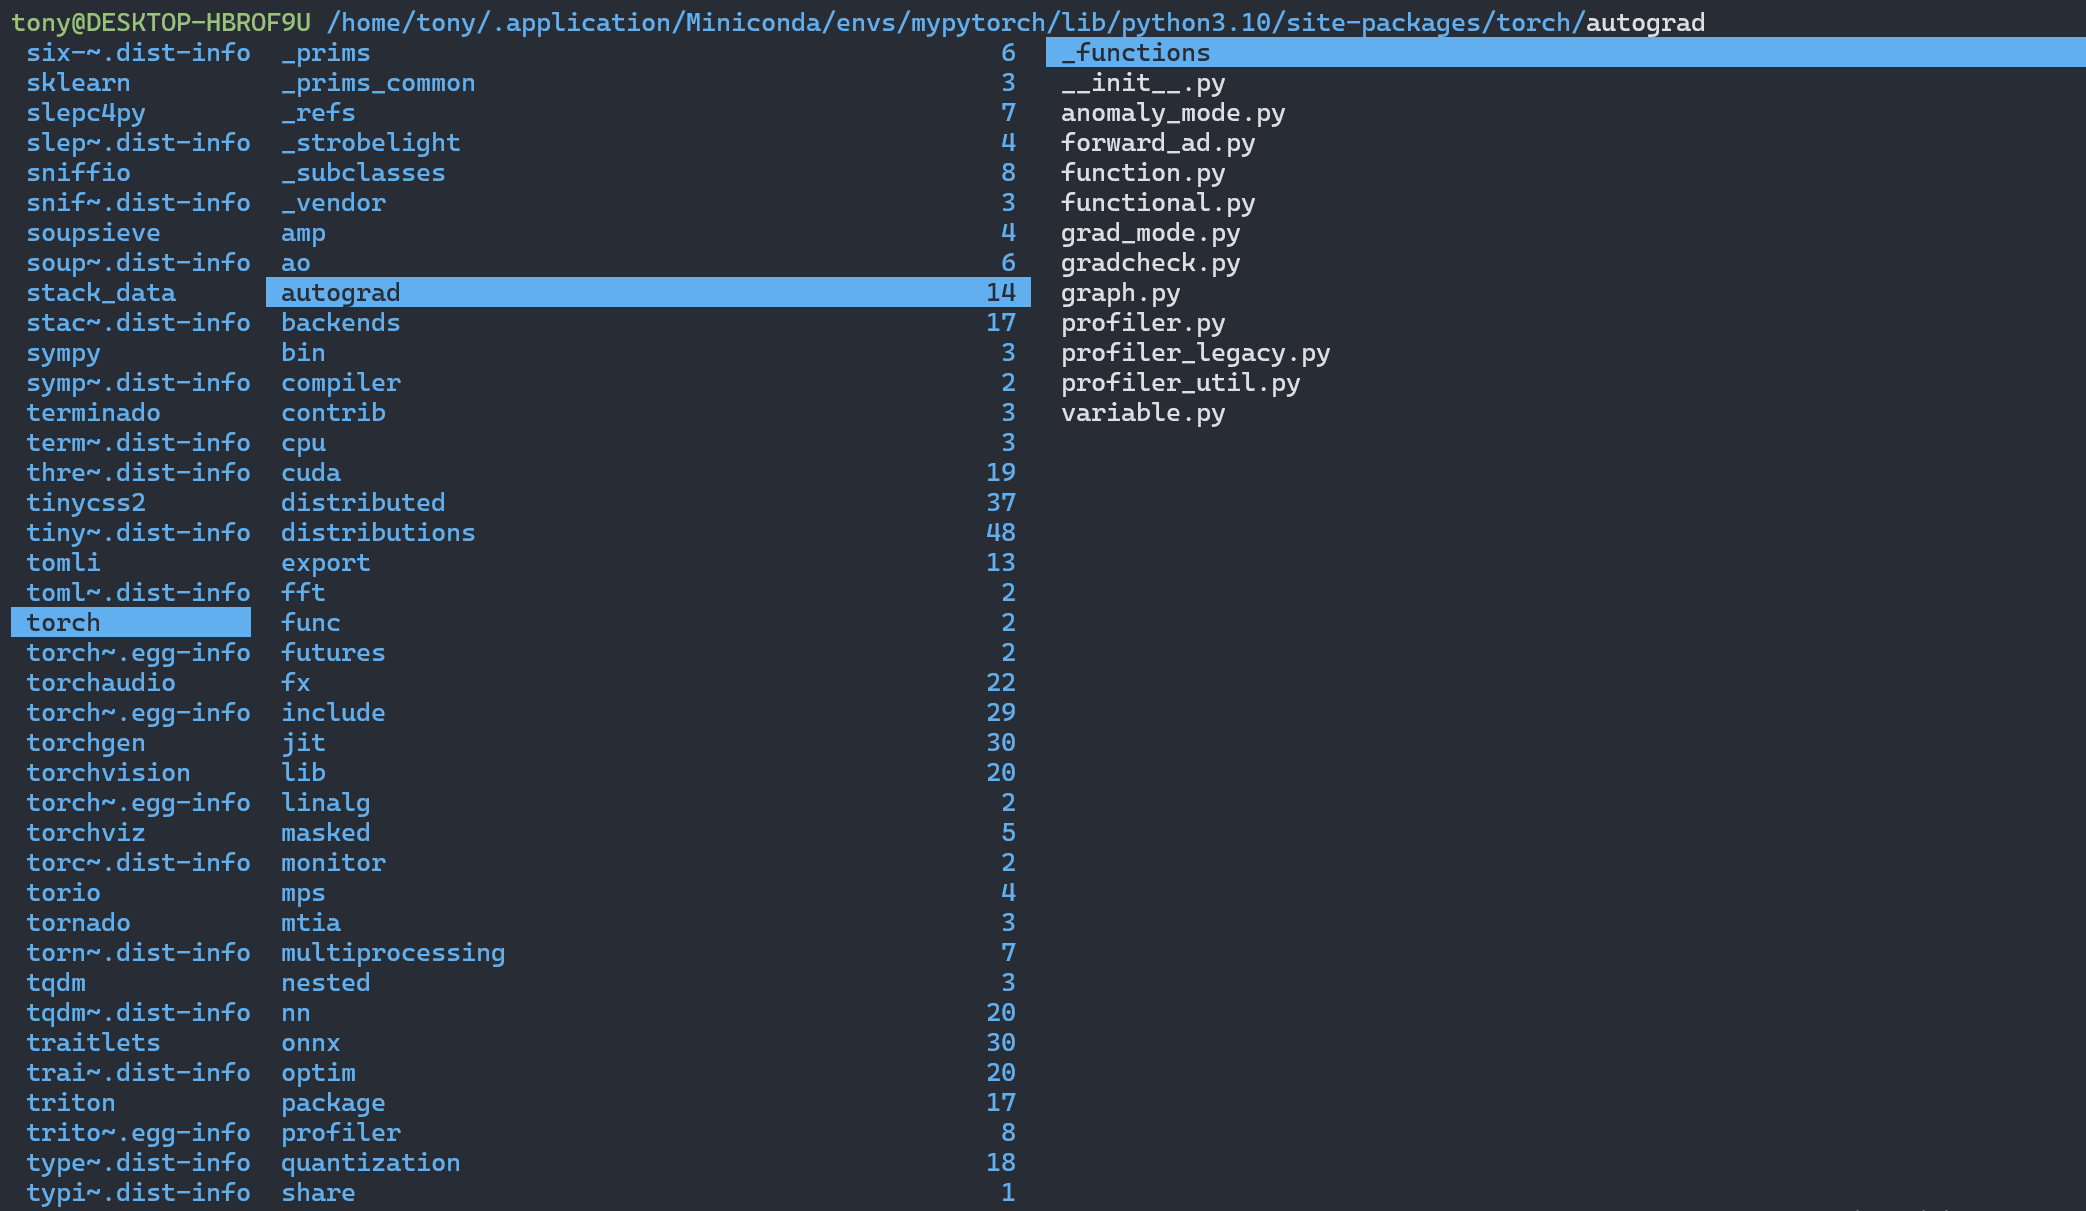
\includegraphics[width=0.6\textwidth]{part/人工智能/深度学习框架/pic/Pytorch/PyTorch概述/PyTorch安装目录.png}
    \caption{PyTorch安装目录}
    \label{fig:PyTorch安装目录}
\end{figure}

\subsubsection{PyTorch的主要模块}
\begin{enumerate}[label=\arabic*)]
    \item \_C

    从文件夹名称就知道它和C语言有关，其实它是辅助C语言代码调用的一个模块，该文件夹里存放了一系列pyi文件，
    pyi文件是python用来校验数据类型的，如果调用数据类型不规范，会报错。
    
    PyTorch的底层计算代码采用的是C++语言编写，并封装成库，供pytorch的python语言进行调用。
    这一点非常重要，后续我们会发现一些pytorch函数无法跳转到具体实现，这是因为具体的实现通过C++语言，我们无法在Pycharm中跳转查看。

    \item include
    
    上面讲到pytorch许多底层运算用的是C++代码，那么C++代码在哪里呢？
    它们在这里,在torch/csrc文件夹下可以看到各个\codeinline{.h/.hpp}文件，而在python库中，只包含头文件，这些头文件就在include文件夹下。

    但如果直接下载的是PyTorch的whl文件，是没有这个文件夹的，因为这个文件夹是源码编译的时候才会有的。

    \item lib
    
    torch文件夹中最重要的一个模块，torch文件夹占3.2GB的空间，98\%的内容都在lib中，占了3.16GB空间。
    pytorch的内容几乎都在lib里面，让我们看看里面是什么。
    
    lib文件夹下包含大量的.lib .so文件（分别是静态链接库和动态链接库），例如大名鼎鼎的\codeinline{libcudnn\_*.so}， \codeinline{libc*\_cuda.so}。
    这些底层库都会被各类顶层python api调用。

    \item autograd：自动求导，自动计算张量的梯度，用于反向传播
    
    该模块是pytorch的核心模块与概念，它实现了梯度的自动求导，
    极大地简化了深度学习研究者开发的工作量，开发人员只需编写前向传播代码，反向传播部分由\codeinline{autograd}自动实现，
    再也不用手动去推导数学公式，
    然后编写代码了（很多朋友可能不知道，在早期的深度学习框架中是没有这个功能的，例如caffe，它需要手动编写反向传播的公式代码）
    \begin{figure}[htpb]
        \centering
        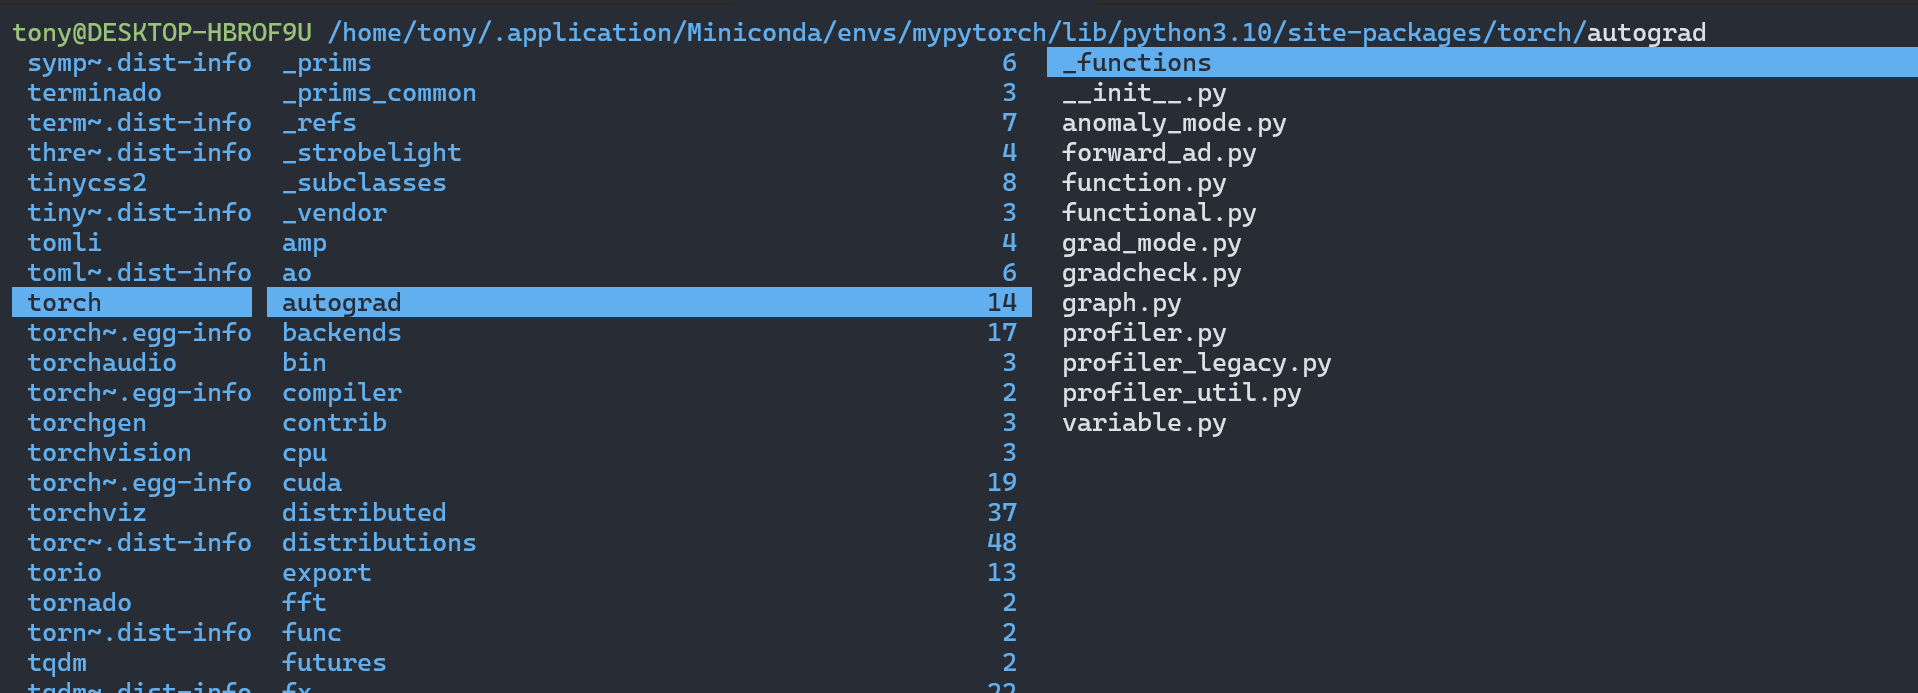
\includegraphics[width=0.6\textwidth]{part/人工智能/深度学习框架/pic/Pytorch/PyTorch概述/autograd中的算法.png}
        \caption{autograd中的算法}
        \label{fig:autograd中的算法}
    \end{figure}
    
    
    \item nn：神经网络模块
    
    相信这个模块是99\%pytorch开发者使用频率最高的模块，
    搭建网络的网络层就在\codeinline{nn.modules}里边。
    我们可以到\codeinline{torch/nn/modules}里面看常用的网络层，
    包括常见的层（如全连接层、卷积层、循环层等）以及损失函数。
    
    \begin{figure}[htpb]
        \centering
        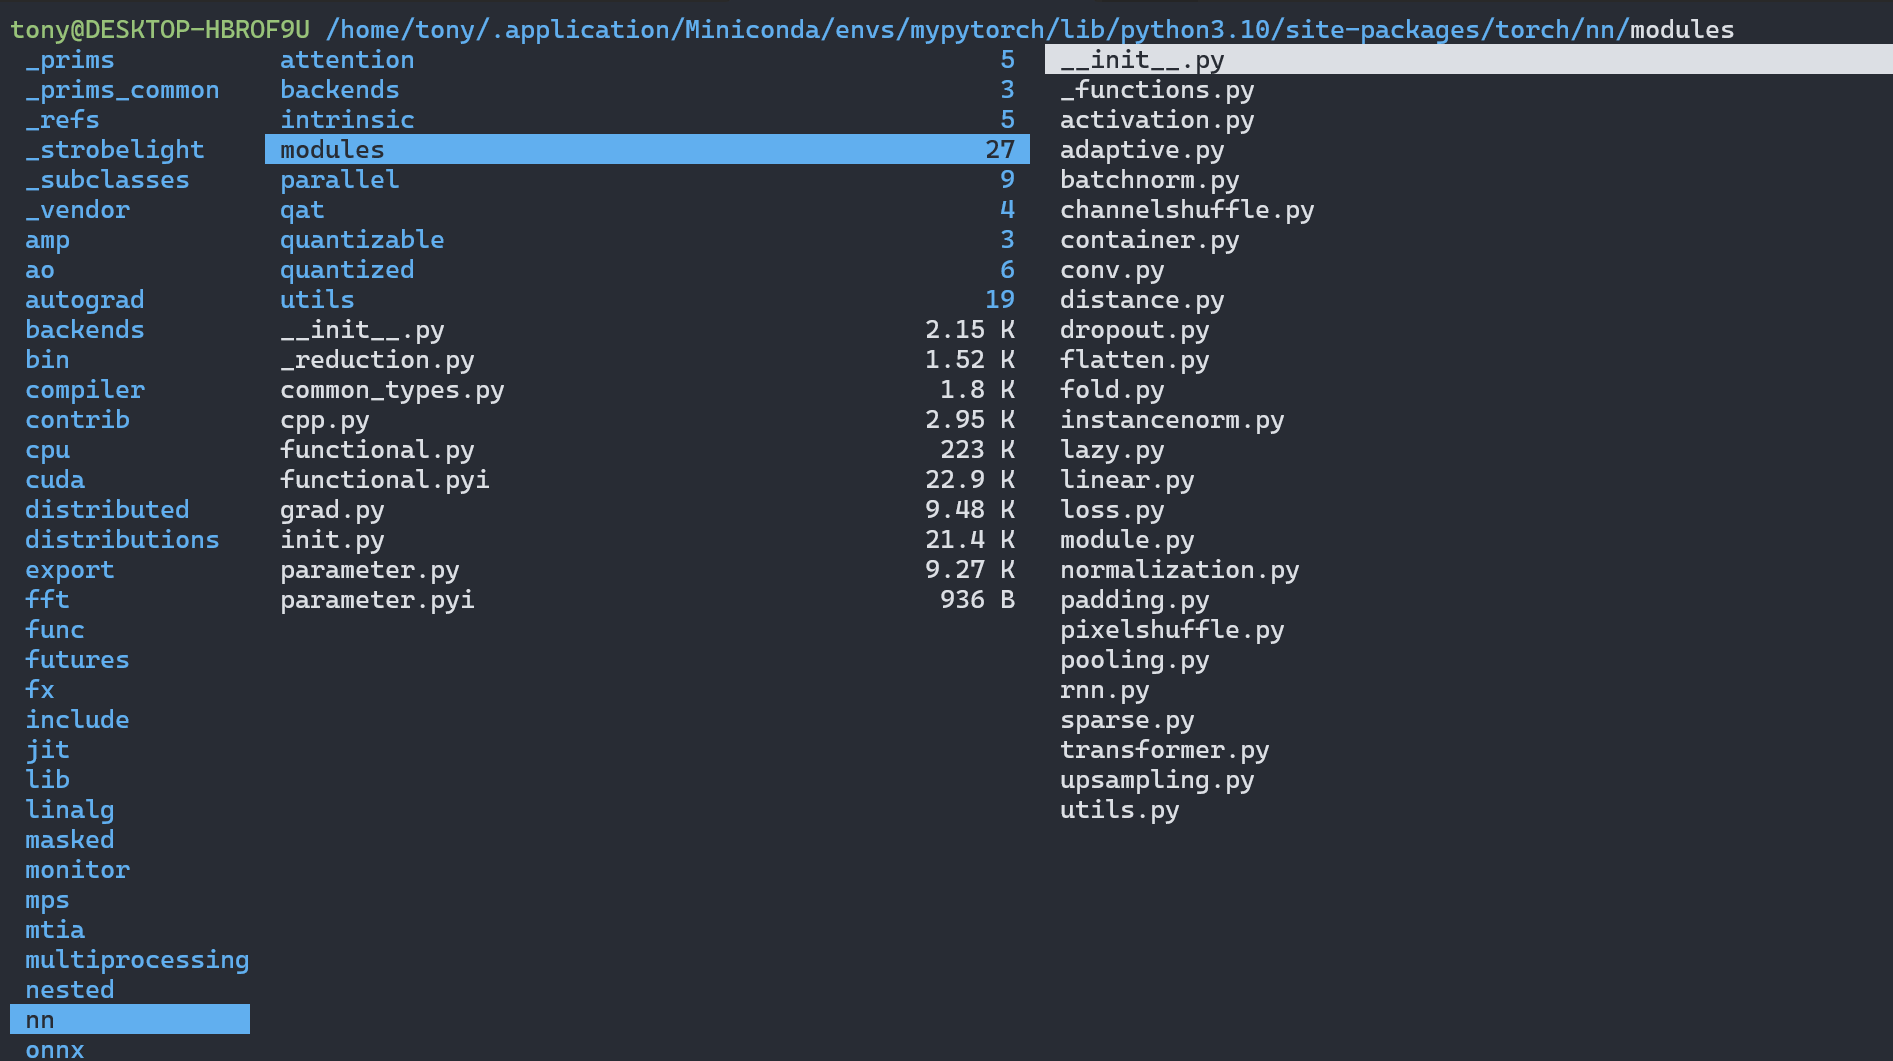
\includegraphics[width=0.6\textwidth]{part/人工智能/深度学习框架/pic/Pytorch/PyTorch概述/nn.modules中的网络层.png}
        \caption{nn.modules中的网络层}
        \label{fig:nn.modules中的网络层}
    \end{figure}
    

    \item onnx
    
    pytorch模型转换到onnx模型表示的核心模块，
    进入文件夹可以看到大量的\codeinline{opset**.py}，

    \item optim
    
    优化模块，深度学习的学习过程，就是不断的优化，而优化使用的方法函数，
    都暗藏在了optim文件夹中，进入该文件夹，
    可以看到熟悉的优化方法：“Adam”、“SGD”、“ASGD”等。以及非常重要的学习率调整模块，\codeinline{lr\_scheduler.py}。
    
    \begin{figure}[htpb]
        \centering
        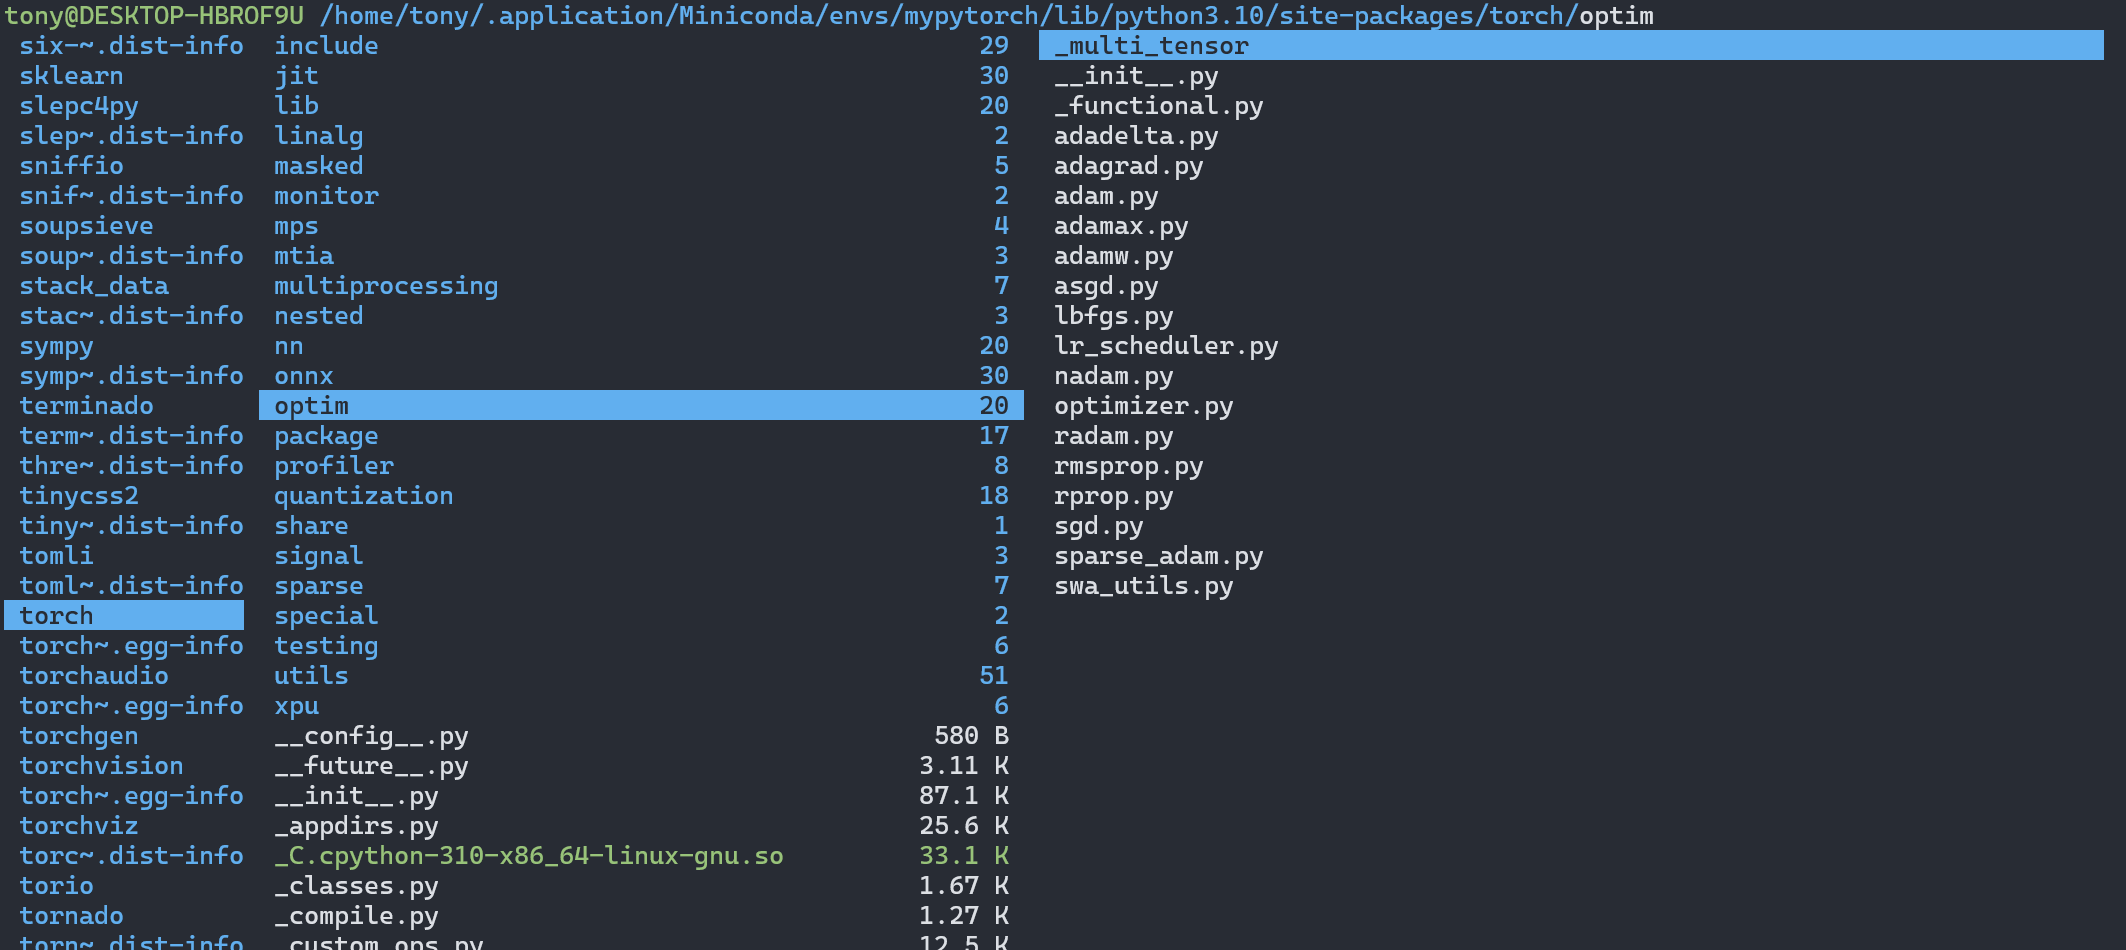
\includegraphics[width=0.6\textwidth]{part/人工智能/深度学习框架/pic/Pytorch/PyTorch概述/optim中的算法.png}
        \caption{optim中的算法}
        \label{fig:optim中的算法}
    \end{figure}
    

    \item utils
    
    utils是各种软件工程中常见的文件夹，其中包含了各类常用工具，
    其中比较关键的是data文件夹，tensorboard文件夹，
    这些工具都将在后续章节详细展开。
\end{enumerate}


\subsection{torchvision 相关}
\label{subsec:torchvision相关}
专门为计算机视觉任务设计的附加库，扩展了 PyTorch 的功能。

\subsubsection{torchvision 安装目录}
\label{subsubsec:torchvision安装目录}
\begin{figure}[htpb]
    \centering
    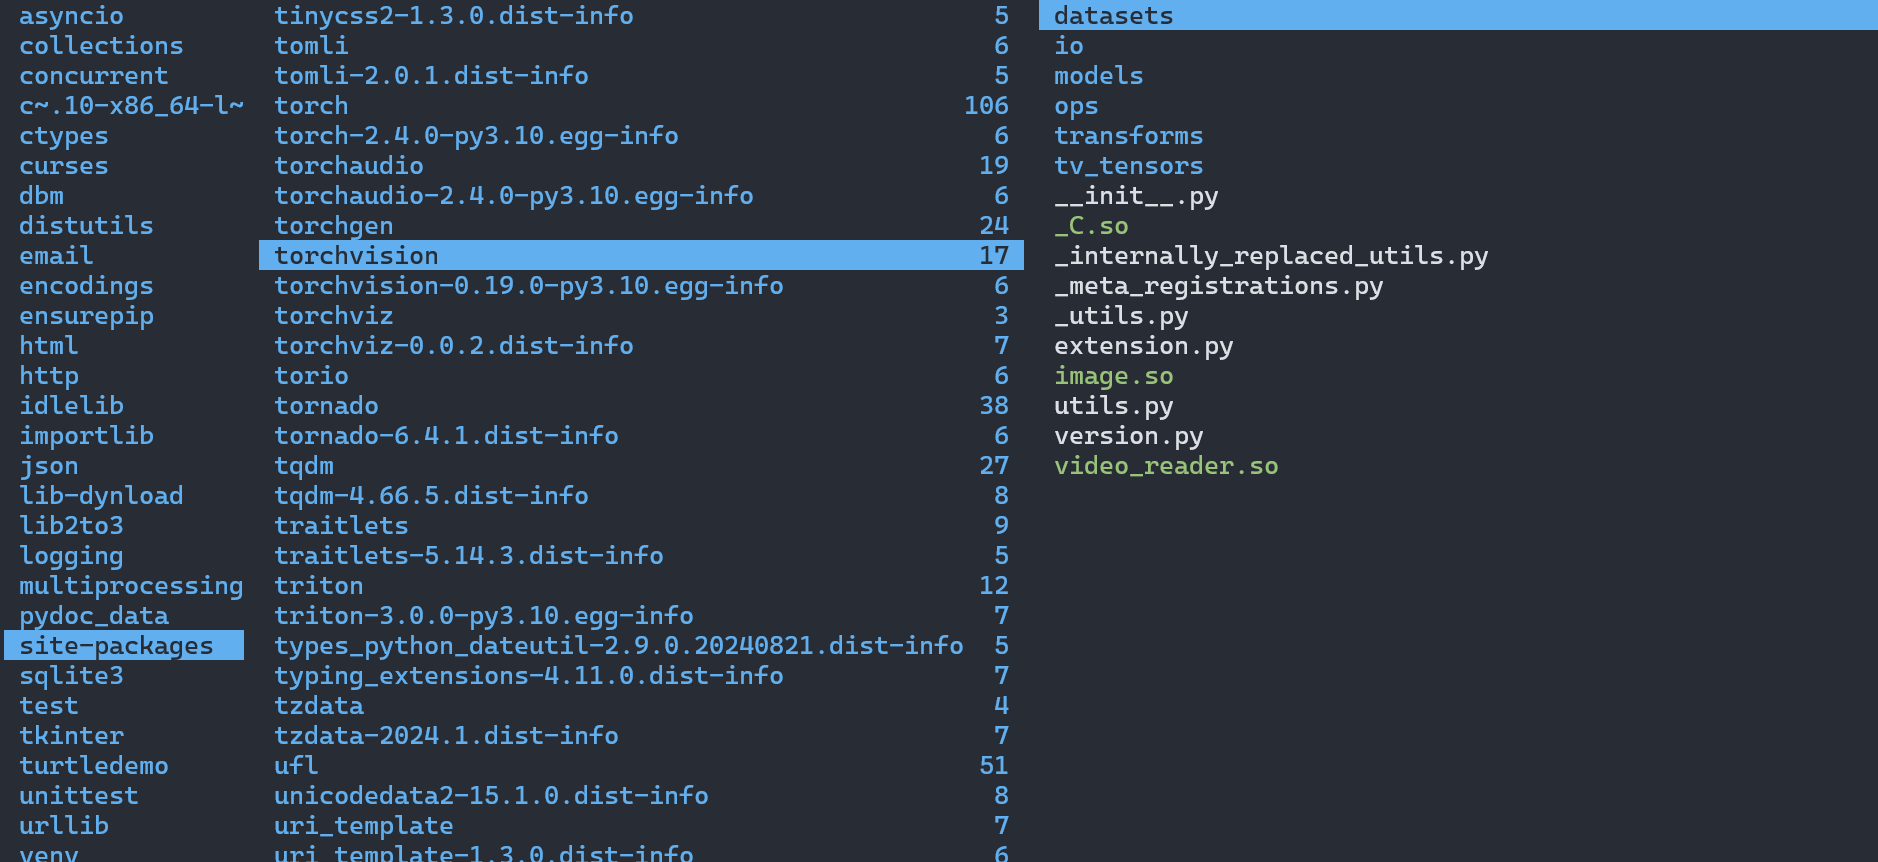
\includegraphics[width=0.6\textwidth]{part/人工智能/深度学习框架/pic/Pytorch/PyTorch概述/torchvision的安装目录.png}
    \caption{torchvision的安装目录}
    \label{fig:torchvision的安装目录}
\end{figure}

\subsubsection{torchvision的主要模块}
\label{subsubsec:torchvision的主要模块}
\begin{enumerate}[label=\arabic*)]
    \item datasets
    
    提供了一系列常用的计算机视觉数据集的接口，如 CIFAR-10、ImageNet、MNIST 等。用户可以通过简单的 API 下载、加载和预处理这些数据集。

    \begin{figure}[htpb]
        \centering
        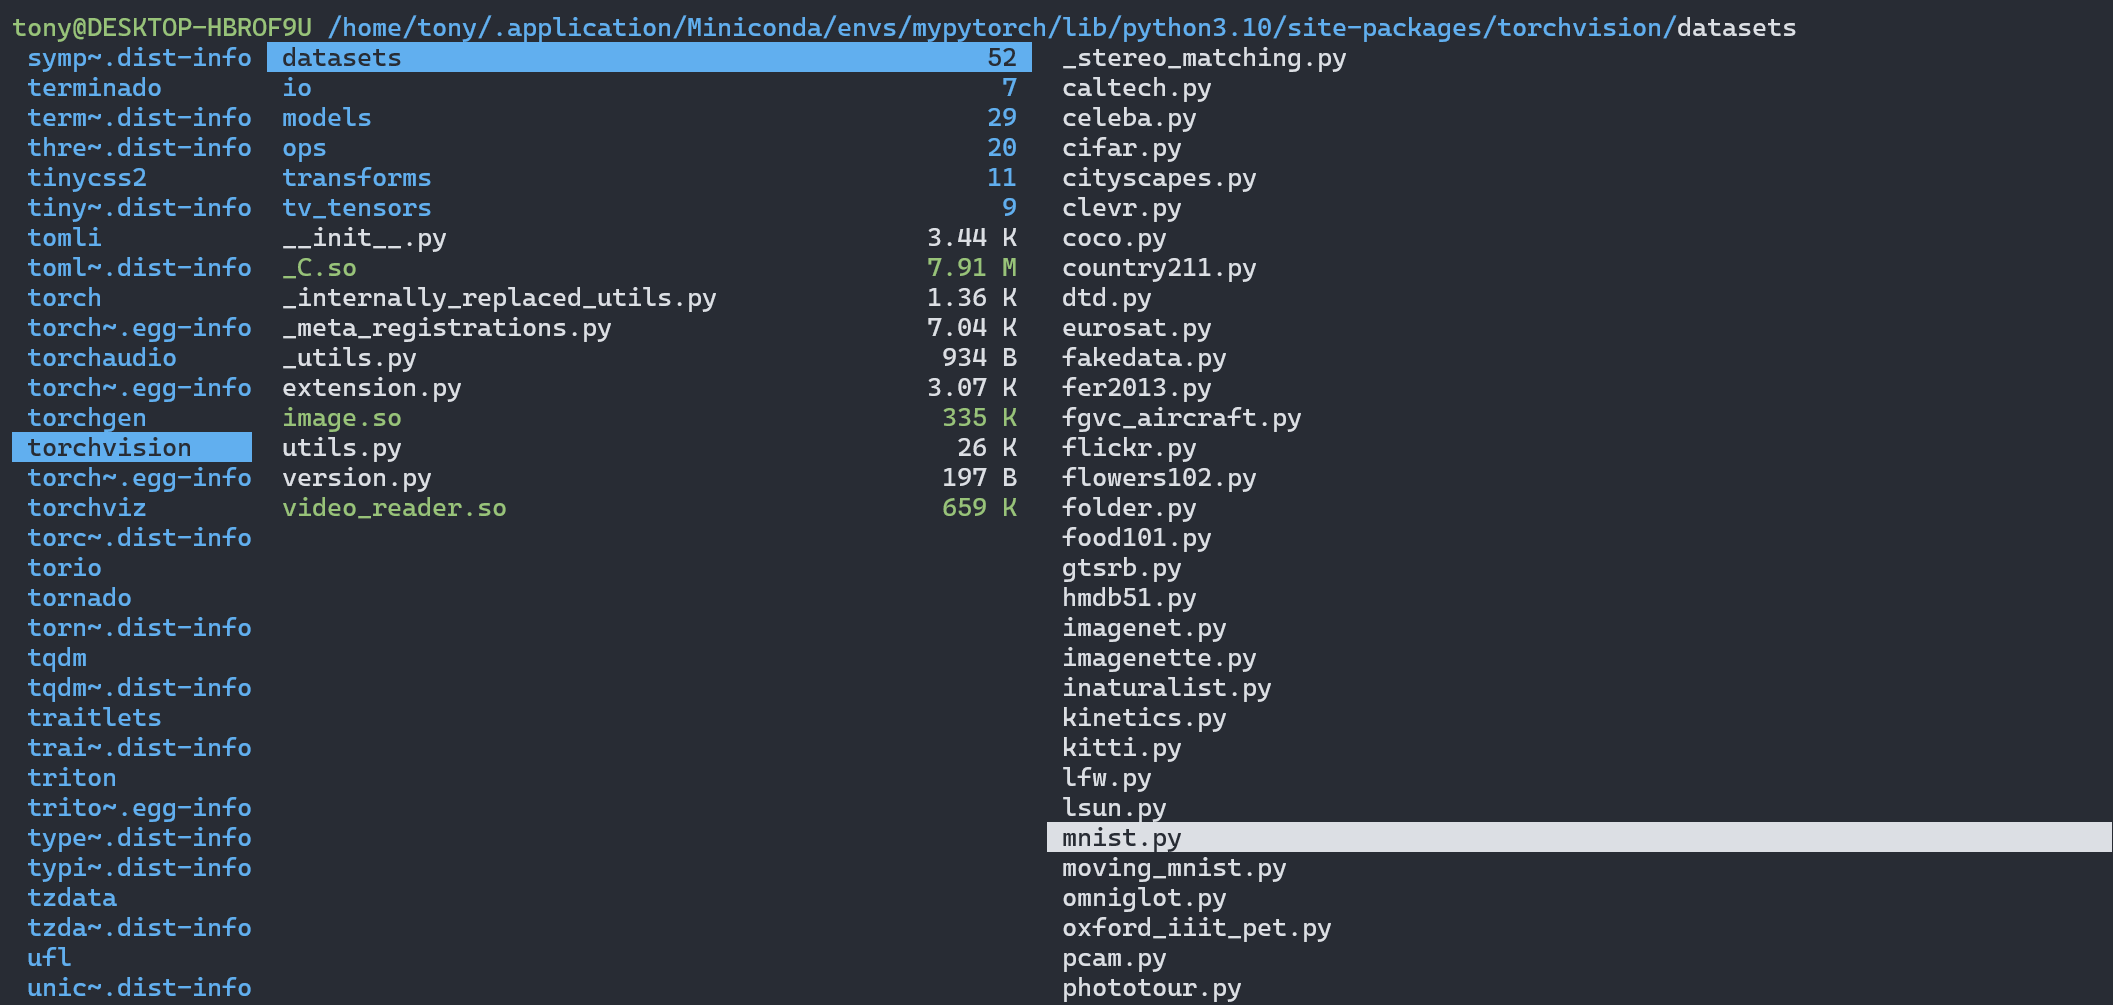
\includegraphics[width=0.6\textwidth]{part/人工智能/深度学习框架/pic/Pytorch/PyTorch概述/datasets内容.png}
        \caption{datasets内容}
        \label{fig:datasets内容}
    \end{figure}
    
    \item models:预训练模型
    
    这里是宝藏库，里边存放了经典的、可复现的、有训练权重参数可下载的视觉模型，
    例如分类的alexnet、densenet、efficientnet、mobilenet-v1/2/3、resnet等，
    分割模型、检测模型、视频任务模型、量化模型。
    

    \item ops
    
    视觉任务特殊的功能函数，例如检测中用到的 roi\_align, roi\_pool，boxes的生成，以及focal\_loss实现，都在这里边有实现。

    \item transforms:图像转换
    
    提供了一系列常用的图像预处理方法。数据增强，数据预处理，数据增强的函数都在这里，
    例如缩放(resize), 裁剪(crop), 归一化(normalize), 旋转(rotate), 翻转(flip)等。

    通过\codeinline{torchvision/transforms/transforms.py}, 可以看到 torchvision包含了这些功能

    \begin{lstlisting}[style=demostyle,numbers=none]
    __all__ = ["Compose", "ToTensor", "PILToTensor", "ConvertImageDtype", "ToPILImage", "Normalize", "Resize", "Scale",
           "CenterCrop", "Pad", "Lambda", "RandomApply", "RandomChoice", "RandomOrder", "RandomCrop",
           "RandomHorizontalFlip", "RandomVerticalFlip", "RandomResizedCrop", "RandomSizedCrop", "FiveCrop", "TenCrop",
           "LinearTransformation", "ColorJitter", "RandomRotation", "RandomAffine", "Grayscale", "RandomGrayscale",
           "RandomPerspective", "RandomErasing", "GaussianBlur", "InterpolationMode", "RandomInvert", "RandomPosterize",
           "RandomSolarize", "RandomAdjustSharpness", "RandomAutocontrast", "RandomEqualize"]
    \end{lstlisting}
\end{enumerate}










